%% The following is a directive for TeXShop to indicate the main file
%%!TEX root = diss.tex

\chapter{Theory}
\label{ch:Theory}

\section{Cherenkov Radiation}
While the speed of light in a vacuum is fixed as $c$, when light passes through a medium with a refractive index of $n$, it will travel at the velocity $\frac{c}{n}$.
When a charged particle travels through a dielectric medium at a velocity greater than the speed of light in the medium, it will emit Cherenkov radiation \cite{cherenkov}.
As the charged particle travels through the medium (known as a radiator), it will displace electrons, emitting photons radially at points along the particle's path.
If we define the particle velocity to be $v_p$ and $\beta = v_p / c$, then in a time $t$, the particle will travel a distance $\beta ct$.
In that same amount of time, the photons emitted in the radiator have to travel a distance $(c/n)t$.
The geometry of this emission is shown in in Figure \ref{fig:cherenkov}.
This creates a wavefront of light emitted obeying the following relation:
\begin{equation}
    cos(\theta) = \frac{1}{\beta n}
    \label{eq:cherenkovAngle}
\end{equation}

\begin{figure}[]
\centering
\resizebox{0.8\textwidth}{!}{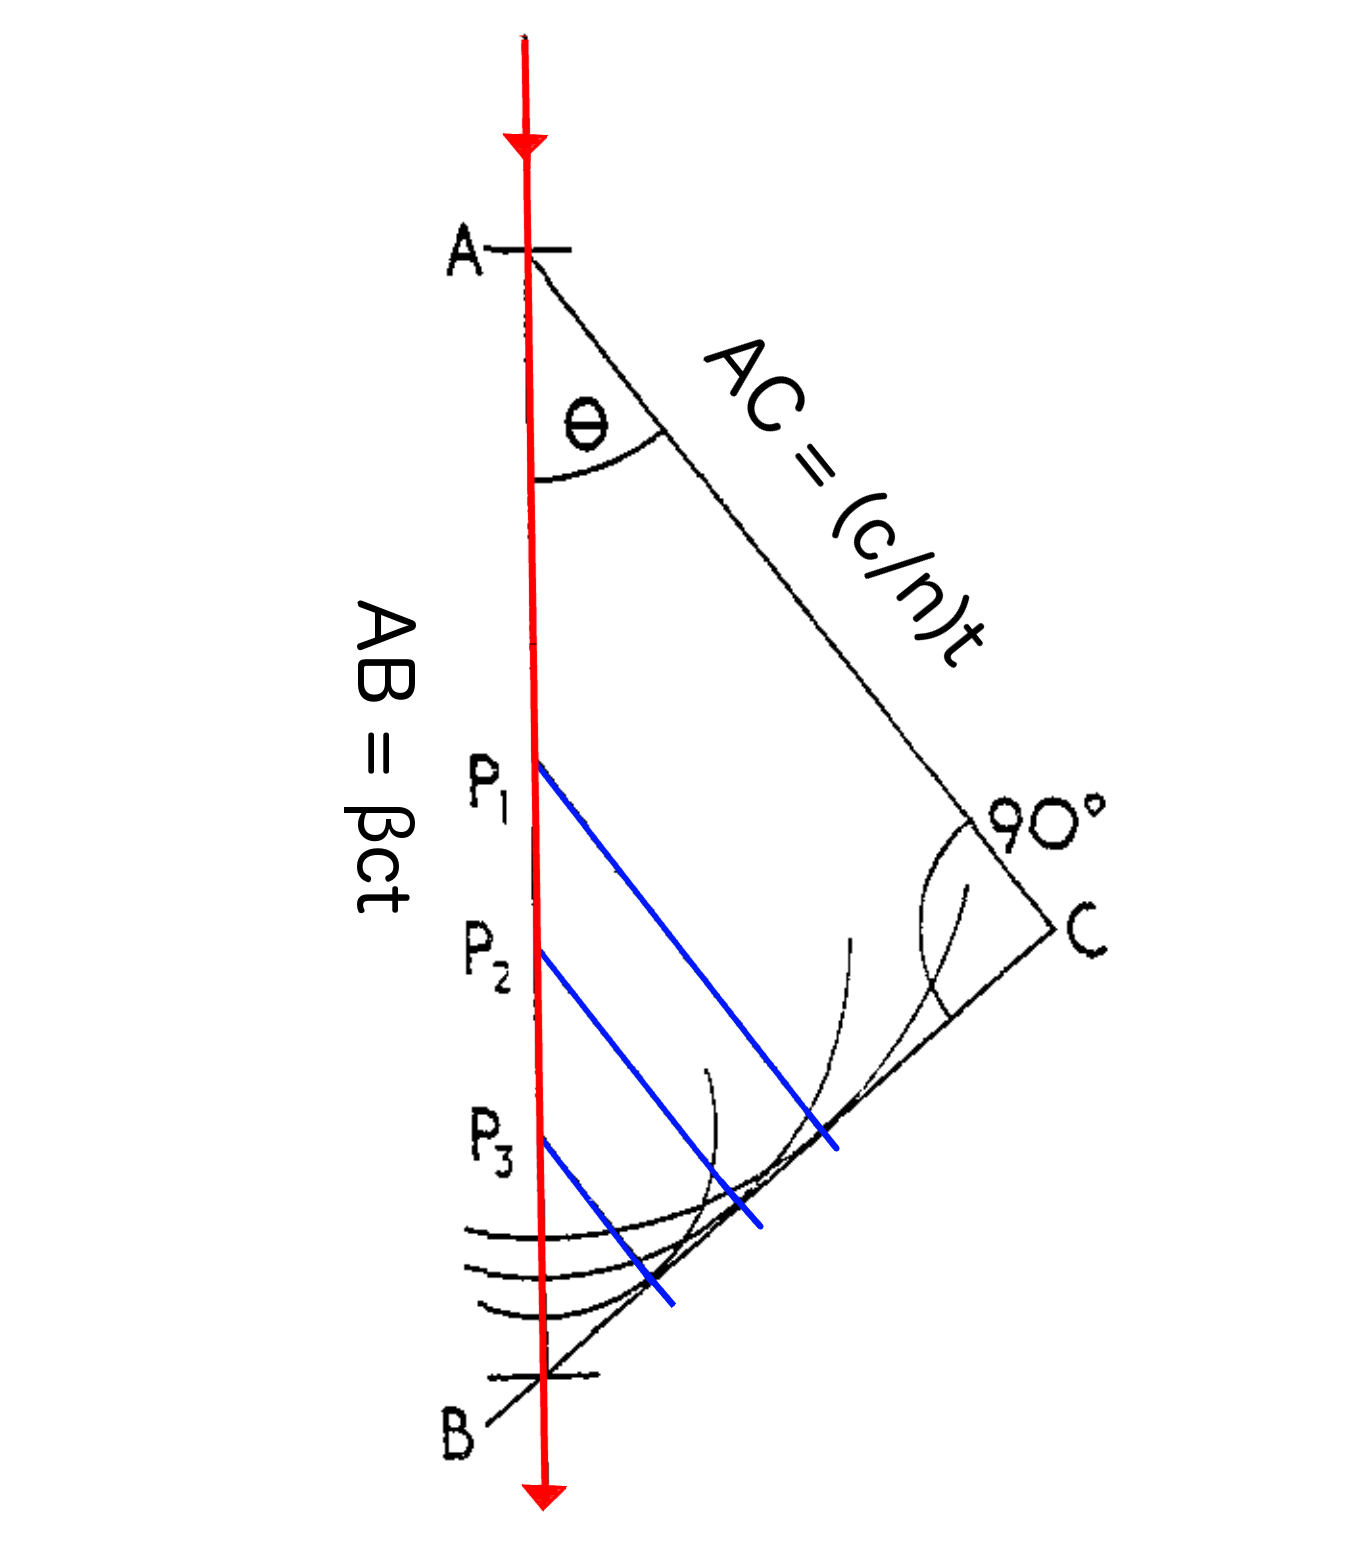
\includegraphics{./figs/cherenkovMod.png}}
\caption[Diagram showing the emission of Cherenkov radiation]{Diagram showing the emission of Cherenkov radiation, adapted from \cite{cherenkov}.
In this diagram, a particle travels along the vertical line from point A to point B.
Electromagnetic radiation is emitted at $P_1$, $P_2$, and $P_3$, each producing one of the curves shown.
It can be seen that these emissions all produce a wavefront along BC, giving a common angle of emission $\theta$.}
\label{fig:cherenkov} 
\end{figure}

This simple relation between photon angle and particle velocity is complicated by the dependency of the refractive index of a medium on the wavelength of light, which must be determined experimentally for a given radiator.

The energy emitted via Cherenkov radiation by a particle of charge $q$ as it moves a distance $dl$ is given by the Frank-Tamm formula \cite{frankTamm}:
\begin{equation}
    \label{eq:frankTamm}
    \frac{dW}{dl} = \frac{q^2}{c^2}\int_{\beta n > 1} \omega  \left(1 - \frac{1}{\beta^2n(\omega)^2}\right)d\omega
\end{equation}

In this formula, $\omega$ is the angular frequency of the light.
If we neglect the frequency dependence of the index of refraction, then we can use this equation to extract the expected number of photons emitted per length $dl$ over a range of frequencies from $\lambda_1$ to $\lambda_2$:

\begin{equation}
    \label{eq:photonNumber}
    \frac{dN}{dl}  = 2\pi\alpha q^2 \left(\frac{1}{\lambda_2} - \frac{1}{\lambda_1}
    \right)\left(1 - \frac{1}{\beta^2n^2}\right)
\end{equation}

Here, $\alpha$ is the fine structure constant ($\approx \frac{1}{137}$).



\section{Aerogel Ring Imaging Cherenkov Detectors}
\label{sec:ARICH}
The relationship between particle velocity through a radiator and photon angle of emission (Equation \ref{eq:cherenkovAngle}) can be exploited for particle identification.
An \ac{ARICH} detector consists of a silica aerogel radiator, and an array of \ac{PMT}s, which can detect the Cherenkov radiation.
Silica aerogel is a substance made of a network of silica (SiO$_2$) clusters interspersed with nanopores of air \cite{aerogelRefraction}.
During production, the refractive index of aerogel can be precisely tuned \cite{aerogelRefraction}, and the wavelength-dependency of the refractive index is  understood \cite{aerogelWavelength}. 

High-velocity hadrons produced in the collision of the proton beam with a target will emit cones of Cherenkov radiation as they travel through the aerogel, leading to an elliptically shaped set of detected photons.
With a known separation distance between the radiator and the detector, the angle of emission $\theta$ of a photon may be determined, which yields the velocity of the particle.
By averaging over several photons emitted by a single particle, we can increase our angular resolution.
With a thicker slab of aerogel, a charged particle travels a greater distance and is likely to emit a greater number of photons.
However, this means that the point of emission of the photon can vary more, leading to lower angular resolution.
To combat this, \ac{ARICH} detectors can use two or more layers of aerogel with differing indices of refraction, with the layer closest to the detector having a higher index of refraction \cite{belleArich}.
The photons emitted in the first layer will be emitted at a smaller angle than those from the second layer, and ultimately arrive on the same ring on the photon detector array.

The \ac{PMT}s used in the detectors function by creating a rapid cascade of electrons and a corresponding signal upon being struck by a photon.
Their quantum efficiencies depend on the wavelength of the incident light, and are well-characterized by the manufacturer.


\endinput

Any text after an \endinput is ignored.
You could put scraps here or things in progress.
